\documentclass[12pt]{article} % use larger type; default would be 10pt

\usepackage{tikz}
\usepackage{pgfplots}
\usetikzlibrary{calc}
\usetikzlibrary{arrows.meta}
\usetikzlibrary{patterns}
        \newcommand\degree[0]{^{\circ}}
\usetikzlibrary{shapes.misc}

\title{Play with TikZ}
\author{Just Us}
%\date{} % Activate to display a given date or no date (if empty),
         % otherwise the current date is printed 

\begin{document}
\maketitle

\section{Chap 5 Equations and Identities}

\subsection{5.3 Trigonometric Identities}

fig-5-3-abs $y=\sqrt{x^2}$ and $y=x$
\begin{tikzpicture} [scale=.5]
\coordinate (O) at (0,0);
\coordinate (B) at ($ (O)+(0,-4) $);
\draw[black, thick] (O)++(-4.7,0)--++(9.4,0);
\draw[black, thick] (O)++(0,-3.1)--++(0,6.2);
\draw[blue, thick] (O)++(-3.1,3.1)--(O)--++(3.1,3.1);
\node[text width = 1.8cm] at (B) {\color{blue}$Y_1=\sqrt{x^2}$};

\coordinate (O) at (11,0);
\coordinate (B) at ($ (O)+(0,-4) $);
\draw[black, thick] (O)++(-4.7,0)--++(9.4,0);
\draw[black, thick] (O)++(0,-3.1)--++(0,6.2);
\draw[blue, thick] (O)++(-3.1,-3.1)--(O)--++(3.1,3.1);
\node[text width = 1.4cm] at (B) {\color{blue}$Y_2=x$};
\end{tikzpicture}
\newline

fig-5-3-abs v2 $y=\sqrt{x^2}$ and $y=x$
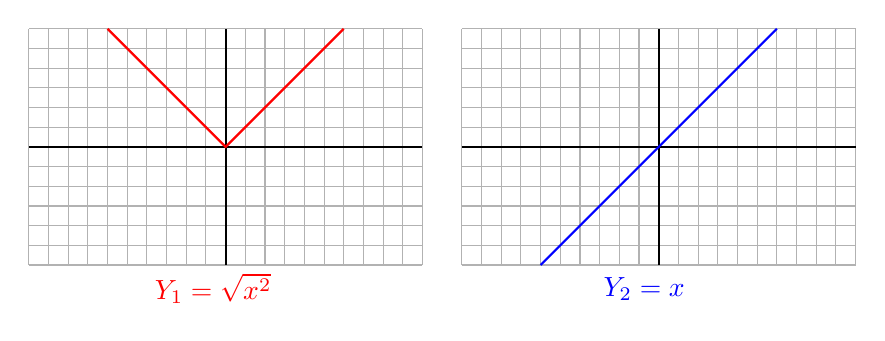
\begin{tikzpicture} [scale=.25]

\draw[gray!60] (-10,-6) grid (10,6);
\coordinate (O) at (0,0);
\coordinate (B) at ($ (O)+(0,-7.2) $);
\draw[black, thick] (O)++(-10,0)--++(20,0);
\draw[black, thick] (O)++(0,-6)--++(0,12);
\draw[red, thick] (O)++(-6,6)--(O)--++(6,6);
\node[text width = 1.8cm] at (B) {\color{red}$Y_1=\sqrt{x^2}$};

\draw[gray!60] (12,-6) grid (32,6);
\coordinate (O) at (22,0);
\coordinate (B) at ($ (O)+(0,-7.2) $);
\draw[black, thick] (O)++(-10,0)--++(20,0);
\draw[black, thick] (O)++(0,-6)--++(0,12);
\draw[blue, thick] (O)++(-6,-6)--(O)--++(6,6);
\node[text width = 1.4cm] at (B) {\color{blue}$Y_2=x$};
\end{tikzpicture}
\newline

fig-5-3-abs v2 $y=\sqrt{x^2}$ and $y=x$
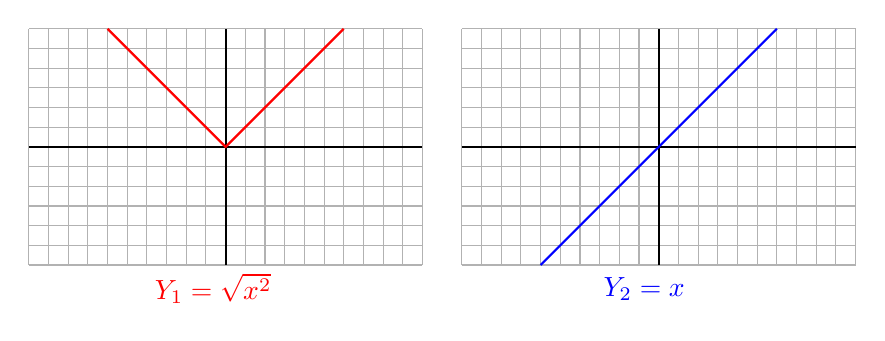
\begin{tikzpicture} [scale=.25]

\draw[gray!60] (-10,-6) grid (10,6);
\coordinate (O) at (0,0);
\coordinate (B) at ($ (O)+(0,-7.2) $);
\draw[black, thick] (O)++(-10,0)--++(20,0);
\draw[black, thick] (O)++(0,-6)--++(0,12);
\draw[red, thick] (O)++(-6,6)--(O)--++(6,6);
\node[text width = 1.8cm] at (B) {\color{red}$Y_1=\sqrt{x^2}$};

\draw[gray!60] (12,-6) grid (32,6);
\coordinate (O) at (22,0);
\coordinate (B) at ($ (O)+(0,-7.2) $);
\draw[black, thick] (O)++(-10,0)--++(20,0);
\draw[black, thick] (O)++(0,-6)--++(0,12);
\draw[blue, thick] (O)++(-6,-6)--(O)--++(6,6);
\node[text width = 1.4cm] at (B) {\color{blue}$Y_2=x$};
\end{tikzpicture}
\newline




\section {Stuff for later}




sine graph
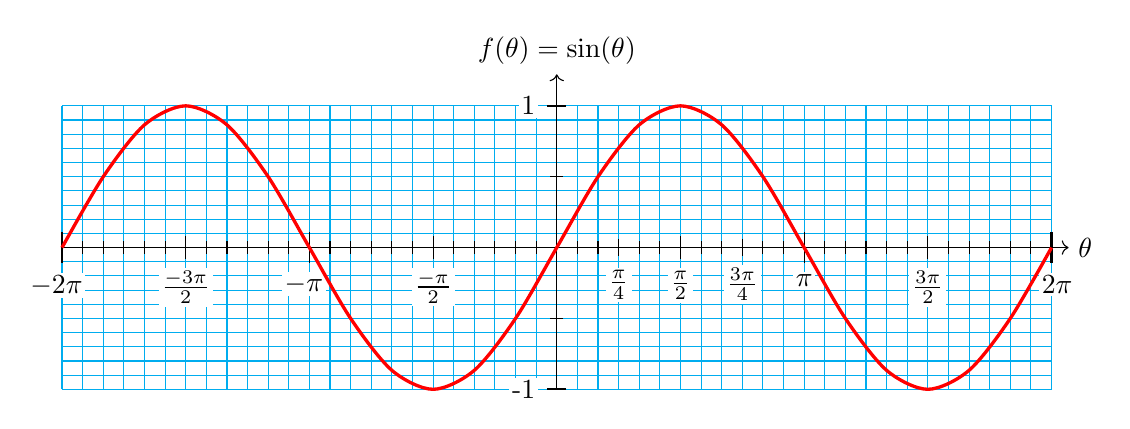
\begin{tikzpicture}

\draw[cyan,xstep=pi/12,ystep=0.18]
(-2*pi,-1.8) grid (2*pi,1.8);

\draw[->] (-6.3,0) -- (6.5,0) node[right] {$\theta$};
\draw[->] (0,-1.8) -- (0,2.2) node[above] {$f(\theta)=\sin(\theta)$};

\foreach \x in {-24,-23,...,24}
\draw[black] ($ pi*\x /12*(1,0) +(0,.08) $) --++(0,-.16);
\foreach \y in {-0.9, 0.9}
\draw[black] (.08,\y ) --++(-.16,0);
\foreach \y in {-1,1}
\draw[black, thick] (.12,1.8*\y ) --++(-.24,0) node[anchor=east, xshift=-3, fill=white, inner sep=1pt] {\y};

\draw[black, thick] (-2*pi,.2) --++(0,-.4) node[anchor=north, xshift=-2,yshift=-3, fill=white, inner sep=1pt] {$-2\pi$};
\draw[black, thick] (2*pi,.2) --++(0,-.4) node[anchor=north, xshift=2,yshift=-3, fill=white, inner sep=1pt] {$2\pi$};

\draw[black] (pi,.2) --++(0,-.4) node[anchor=north, yshift=-3, fill=white, inner sep=1pt] {$\pi$};

\draw[black] (pi,.2) --++(0,-.4) node[anchor=north, yshift=-3, fill=white, inner sep=1pt] {$\pi$};
\draw[black] (-pi,.2) --++(0,-.4) node[anchor=north, xshift=-2,yshift=-3, fill=white, inner sep=1pt] {$-\pi$};
\draw[black] (-pi/2,.15) --++(0,-.3) node[anchor=north, yshift=-3, fill=white, inner sep=1pt] {$\frac{-\pi}{2}$};
\draw[black] (pi/2,.15) --++(0,-.3) node[anchor=north, yshift=-3, fill=white, inner sep=1pt] {$\frac{\pi}{2}$};
\draw[black] (3*pi/2,.15) --++(0,-.3) node[anchor=north, yshift=-3, fill=white, inner sep=1pt] {$\frac{3\pi}{2}$};
\draw[black] (-3*pi/2,.15) --++(0,-.3) node[anchor=north, yshift=-3, fill=white, inner sep=1pt] {$\frac{-3\pi}{2}$};

\draw[black] (pi/4,.11) --++(0,-.22) node[anchor=north, yshift=-4, fill=white, inner sep=1pt] {$\frac{\pi}{4}$};

\draw[black] (3*pi/4,.11) --++(0,-.22) node[anchor=north, yshift=-3, fill=white, inner sep=1pt] {$\frac{3\pi}{4}$};

\draw[domain=-2*pi:2*pi,smooth,variable=\x,red,very thick] plot ({\x},{1.8*sin(deg(\x))});

\end{tikzpicture}
\newline


cosine graph
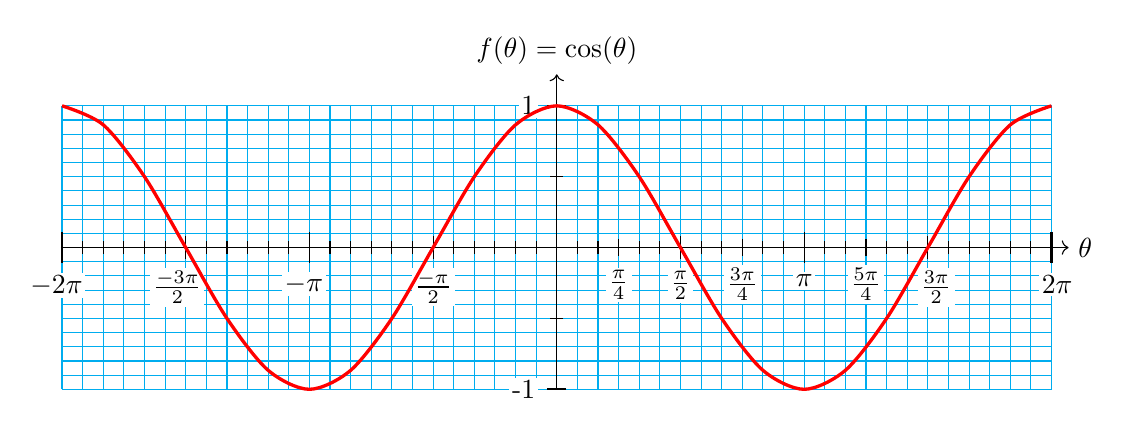
\begin{tikzpicture} 

\draw[cyan,xstep=pi/12,ystep=0.18]
(-2*pi,-1.8) grid (2*pi,1.8);

\draw[->] (-6.3,0) -- (6.5,0) node[right] {$\theta$};
\draw[->] (0,-1.8) -- (0,2.2) node[above] {$f(\theta)=\cos(\theta)$};

\foreach \x in {-24,-23,...,24}
\draw[black] ($ pi*\x /12*(1,0) +(0,.08) $) --++(0,-.16);
\foreach \y in {-0.9, 0.9}
\draw[black] (.08,\y ) --++(-.16,0);
\foreach \y in {-1,1}
\draw[black, thick] (.12,1.8*\y ) --++(-.24,0) node[anchor=east, xshift=-3, fill=white, inner sep=1pt] {\y};

\draw[black, thick] (-2*pi,.2) --++(0,-.4) node[anchor=north, xshift=-2,yshift=-3, fill=white, inner sep=1pt] {$-2\pi$};
\draw[black, thick] (2*pi,.2) --++(0,-.4) node[anchor=north, xshift=2,yshift=-3, fill=white, inner sep=1pt] {$2\pi$};

\draw[black] (pi,.2) --++(0,-.4) node[anchor=north, yshift=-3, fill=white, inner sep=1pt] {$\pi$};

\draw[black] (pi,.2) --++(0,-.4) node[anchor=north, yshift=-3, fill=white, inner sep=1pt] {$\pi$};
\draw[black] (-pi,.2) --++(0,-.4) node[anchor=north, xshift=-2,yshift=-3, fill=white, inner sep=1pt] {$-\pi$};
\draw[black] (-pi/2,.15) --++(0,-.3) node[anchor=north, yshift=-3, fill=white, inner sep=1pt] {$\frac{-\pi}{2}$};
\draw[black] (pi/2,.15) --++(0,-.3) node[anchor=north, yshift=-3, fill=white, inner sep=1pt] {$\frac{\pi}{2}$};
\draw[black] (3*pi/2,.15) --++(0,-.3) node[anchor=north,xshift=3, yshift=-3, fill=white, inner sep=1pt] {$\frac{3\pi}{2}$};
\draw[black] (-3*pi/2,.15) --++(0,-.3) node[anchor=north,xshift=-3, yshift=-3, fill=white, inner sep=1pt] {$\frac{-3\pi}{2}$};

\draw[black] (pi/4,.11) --++(0,-.22) node[anchor=north, yshift=-4, fill=white, inner sep=1pt] {$\frac{\pi}{4}$};

\draw[black] (3*pi/4,.11) --++(0,-.22) node[anchor=north, yshift=-3, fill=white, inner sep=1pt] {$\frac{3\pi}{4}$};

\draw[black] (5*pi/4,.11) --++(0,-.22) node[anchor=north, yshift=-3, fill=white, inner sep=1pt] {$\frac{5\pi}{4}$};

\draw[domain=-2*pi:2*pi,smooth,variable=\x,red,very thick] plot ({\x},{1.8*cos(deg(\x))});

\end{tikzpicture}
\newline


tangent graph
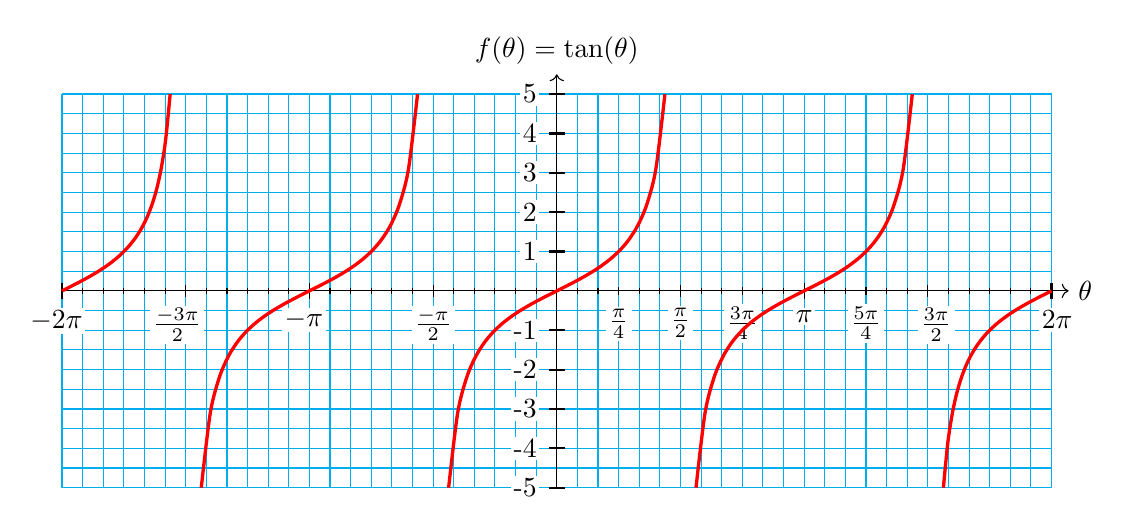
\begin{tikzpicture} [yscale=.5]

\draw[cyan,xstep=pi/12,ystep=0.5]
(-2*pi,-5) grid (2*pi,5);

\draw[->] (-6.3,0) -- (6.5,0) node[right] {$\theta$};
\draw[->] (0,-5) -- (0,5.5) node[above] {$f(\theta)=\tan(\theta)$};

\foreach \x in {-24,-23,...,24}
\draw[black] ($ pi*\x /12*(1,0) +(0,.08) $) --++(0,-.16);
\foreach \y in {-5,-4,...,-1,1,2,...,5}
\draw[black, thick] (.10,\y ) --++(-.2,0) node[anchor=east, xshift=-3, fill=white, inner sep=1pt] {\y};

\draw[black, thick] (-2*pi,.2) --++(0,-.4) node[anchor=north, xshift=-2,yshift=-3, fill=white, inner sep=1pt] {$-2\pi$};
\draw[black, thick] (2*pi,.2) --++(0,-.4) node[anchor=north, xshift=2,yshift=-3, fill=white, inner sep=1pt] {$2\pi$};

\draw[black] (pi,.2) --++(0,-.4) node[anchor=north, yshift=-3, fill=white, inner sep=1pt] {$\pi$};

\draw[black] (pi,.2) --++(0,-.4) node[anchor=north, yshift=-3, fill=white, inner sep=1pt] {$\pi$};
\draw[black] (-pi,.2) --++(0,-.4) node[anchor=north, xshift=-2,yshift=-3, fill=white, inner sep=1pt] {$-\pi$};
\draw[black] (-pi/2,.15) --++(0,-.3) node[anchor=north, yshift=-3, fill=white, inner sep=1pt] {$\frac{-\pi}{2}$};
\draw[black] (pi/2,.15) --++(0,-.3) node[anchor=north, yshift=-3, fill=white, inner sep=1pt] {$\frac{\pi}{2}$};
\draw[black] (3*pi/2,.15) --++(0,-.3) node[anchor=north,xshift=3, yshift=-3, fill=white, inner sep=1pt] {$\frac{3\pi}{2}$};
\draw[black] (-3*pi/2,.15) --++(0,-.3) node[anchor=north,xshift=-3, yshift=-3, fill=white, inner sep=1pt] {$\frac{-3\pi}{2}$};

\draw[black] (pi/4,.11) --++(0,-.22) node[anchor=north, yshift=-4, fill=white, inner sep=1pt] {$\frac{\pi}{4}$};

\draw[black] (3*pi/4,.11) --++(0,-.22) node[anchor=north, yshift=-3, fill=white, inner sep=1pt] {$\frac{3\pi}{4}$};

\draw[black] (5*pi/4,.11) --++(0,-.22) node[anchor=north, yshift=-3, fill=white, inner sep=1pt] {$\frac{5\pi}{4}$};

\foreach \i in {-1, 0, 1}
	\draw[domain={\i*pi-atan(5)*pi/180}:{\i*pi+atan(5)*pi/180}, smooth, variable=\x,red,very thick] plot ({\x},{tan(deg(\x))}) ;

\draw[domain={-2*pi:atan(5)*pi/180-2*pi}, smooth, variable=\x,red,very thick] plot ({\x},{tan(deg(\x))}) ;
\draw[domain={2*pi-atan(5)*pi/180:2*pi}, smooth, variable=\x,red,very thick] plot ({\x},{tan(deg(\x))}) ;

\end{tikzpicture}
\newline


part A: law of sines a circumscribing circle

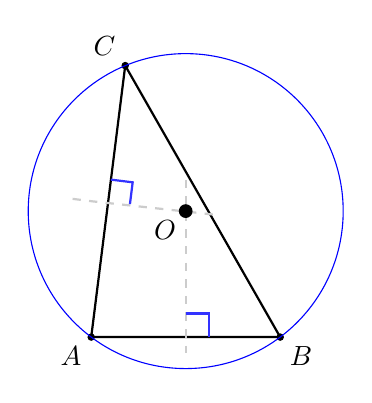
\begin{tikzpicture} [scale=.4]

\coordinate (O) at (0,0);
\coordinate (A) at (-3,-4);
\coordinate (B) at (3,-4);
\coordinate (C) at (-1.92,4.62);

\filldraw (A) circle (.1cm) node[anchor=north east] {$A$};
\filldraw (B) circle (.1cm) node[anchor=north west] {$B$};
\filldraw (C) circle (.1cm) node[anchor=south east] {$C$};

\draw[black,thick] (A)--(B)--(C)--(A);
\draw[gray!40!white, thick, dashed](O)++(0,1) -- (0,-4)--+(0,-.5);
\draw[gray!40!white, thick, dashed](O)++(.862,-.108) -- (-2.96,.31)--++(-.862,.108);
\draw[blue!80!white,thick] (0,-4)++(.75,0)-- ++(0,.75) -- ++(-.75,0);
\draw[blue!80!white,thick] (-2.46,.31) ++(.0864,.6896) -- ++(.6896,-.0864) -- ++(-.0864,-.6896);
\filldraw (O) circle (.2cm) node[anchor=north east] {$O$};

\draw[blue] (O) circle (5);

\end{tikzpicture}
\newline

part B: law of sines a circumscribing circle

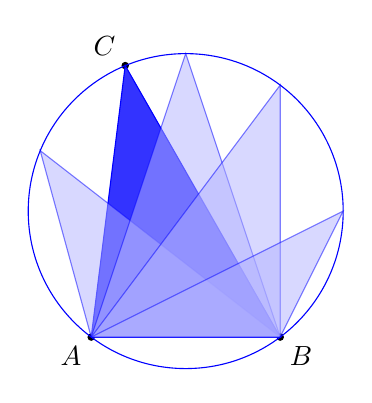
\begin{tikzpicture} [scale=.4]

\coordinate (O) at (0,0);
\coordinate (A) at (-3,-4);
\coordinate (B) at (3,-4);
\coordinate (C) at (-1.92,4.62);
\coordinate (Cp) at (-4.62,1.92);
\coordinate (Cpp) at (0,5);
\coordinate (Cppp) at (3,4);
\coordinate (Cpppp) at (5,0);

\filldraw (O) circle (.1cm) node[anchor=north east] {$O$};
\filldraw (A) circle (.1cm) node[anchor=north east] {$A$};
\filldraw (B) circle (.1cm) node[anchor=north west] {$B$};
\filldraw (C) circle (.1cm) node[anchor=south east] {$C$};

\draw[draw= blue, fill=blue!80!white] (A)--(B)--(C)--(A);
\draw[draw= blue, fill=blue!30!white, opacity=.5] (A)--(B)--(Cp)--(A);
\draw[draw= blue, fill=blue!30!white, opacity=.5] (A)--(B)--(Cpp)--(A);
\draw[draw= blue, fill=blue!30!white, opacity=.5] (A)--(B)--(Cppp)--(A);
\draw[draw= blue, fill=blue!30!white, opacity=.5] (A)--(B)--(Cpppp)--(A);


\draw[blue] (O) circle (5);

\end{tikzpicture}
\newline

Exercise not used?
\begin{tikzpicture}
\coordinate (O) at (0,0);
\coordinate (A) at (0,0);
\coordinate (B) at (0,0);
\coordinate(C) at (0,0);
\coordinate (D) at (0,0);
\filldraw[black] (O) circle (.2pt) node[anchor=south west, xshift=6]{$50\degree$};
\filldraw[black] (A) circle (.2pt) node[anchor=south east]{$x$};
\filldraw[black] (B) circle (.2pt) node[anchor=north east, xshift=-6]{$y$};
\filldraw[black] (C) circle (.2pt) node[anchor=north west]{$z$};
%\draw[black,  thick] (A) -- (B) --( C) -- cycle;
\draw[black] (-2.3,0) --  (2.3,0);
\draw[black] (0.8,1.3) --  (-0.8,-1.3) ;
\end{tikzpicture}
\newline


\end{document}
